\documentclass[11pt,a4paper]{article}

% Page layout
\usepackage[a4paper,margin=2.5cm,top=3cm,bottom=3cm]{geometry}
\usepackage{setspace}
\usepackage{booktabs}
\usepackage{tabularx}

% Typography and fonts
\usepackage[utf8]{inputenc}
\usepackage[T1]{fontenc}
\usepackage{lmodern}

% Graphics and colors
\usepackage{graphicx}
\usepackage{xcolor}
\definecolor{uablue}{RGB}{0,61,165}

% Links and references
\usepackage{hyperref}
\hypersetup{
    colorlinks=true,
    linkcolor=uablue,
    citecolor=uablue,
    urlcolor=uablue,
    bookmarksnumbered=true
}
\usepackage{natbib}
\usepackage{url}

% Diagrams and flowcharts
\usepackage{tikz}
\usetikzlibrary{shapes.geometric, arrows.meta, positioning, calc}

% Code listings
\usepackage{listings}
\lstset{
    basicstyle=\ttfamily\small,
    breaklines=true,
    frame=single,
    numbers=left,
    numberstyle=\tiny\color{gray},
    backgroundcolor=\color{gray!5},
    captionpos=b
}

% Headers and footers
\usepackage{fancyhdr}
\pagestyle{fancy}
\fancyhf{}
\fancyhead[L]{\textcolor{uablue}{Information Retrieval - Assignment 3}}
\fancyhead[R]{\textcolor{uablue}{2025/2026}}
\fancyfoot[C]{\thepage}
\renewcommand{\headrulewidth}{0.4pt}
\renewcommand{\footrulewidth}{0pt}

% Title page
\title{
    \vspace{-1cm}
    \includegraphics[width=0.3\textwidth]{images/logoUantwerpen.png} \\[1cm]
    {\huge\bfseries\textcolor{uablue}{Retrieval Augmented Generation}}\\[0.5cm]
    {\Large Assignment 3}\\[0.3cm]
    {\large Information Retrieval Course}\\
    {\large Academic Year 2025/2026}
}

\author{
    \textbf{Group Members:}\\[0.3cm]
    \begin{tabular}{ll}
        Alperen Davran & s0250946 \\
        Matteo Carlo Comi & s0259766 \\
        Shakhzodbek Bakhtiyorov & s0242661 \\
        Amin Borqal & s0259707 \\
    \end{tabular}\\[1cm]
    \textbf{University of Antwerp}\\
    Faculty of Science\\
    Department of Computer Science
}
\date{
    \today \\[0.5cm]
    \textbf{GitHub Repository:}\\
    \href{https://github.com/alperendavran/Information-Retrieval-Assignment-3}{\textcolor{uablue}{https://github.com/alperendavran/Information-Retrieval-Assignment-3}}
}

\begin{document}

% Title page
\maketitle
\thispagestyle{empty}
\newpage

% Table of contents
\tableofcontents
\newpage

% Set spacing for main content
\onehalfspacing


\section{Introduction}

Retrieval Augmented Generation (RAG) systems combine information retrieval with large language models to provide accurate, grounded answers to user queries. This project implements a RAG system for the University of Antwerp Computer Science Masters program, addressing the challenge of providing prospective and current students with accurate information about courses, prerequisites, schedules, and program requirements.

\subsection{Motivation}

RAG grounds responses in retrieved documents, reduces hallucinations, enables source attribution, and supports knowledge updates without model retraining~\cite{lewis2020}.

\subsection{System Overview}

Our implementation consists of five core components:

\begin{enumerate}
    \item \textbf{Document Chunking}: Splitting course descriptions into semantically coherent passages
    \item \textbf{Embedding \& Indexing}: Computing dense vector representations and building efficient retrieval indices
    \item \textbf{Retrieval Module}: Encoding queries and retrieving top-k similar passages
    \item \textbf{Answer Generation}: Using GPT-4o to synthesize answers from retrieved context
    \item \textbf{Evaluation Framework}: Assessing retrieval quality, answer quality, and error patterns
\end{enumerate}

Our \textbf{main system} (required by the assignment) uses standard dense retrieval with top-k passage selection. We also implemented an \textbf{optional} agentic variant (multi-query expansion, RRF, MMR) as an extra experiment; it is \textit{not} required by the assignment.

\subsection{Assignment Grading Overview}

Table~\ref{tab:grading} maps the assignment's grading criteria to our implementation. Each section fulfils the corresponding requirement.

\begin{table}[h]
\centering
\begin{tabular}{clp{7.5cm}}
\toprule
\textbf{Weight} & \textbf{Component} & \textbf{What We Delivered} \\
\midrule
10\% & Document Chunking (4.1) & 588 passages, 250 tokens/chunk, 15\% overlap, sentence boundaries, preprocessing explained \\
20\% & Embedding \& Indexing (4.2) & all-MiniLM-L6-v2 (local), FAISS Flat, cosine similarity, model justification \\
20\% & Retrieval Module (4.3) & Query encode, top-k=5, rank by similarity, k justified \\
30\% & Answer Generation (4.4) & GPT-4o, natural language query, top-k passages in prompt, RAG vs no-retrieval comparison \\
20\% & System Evaluation (4.5) & Recall@5 (0.796), manual inspection, RAG vs baseline, ≥3 retrieval failures, ≥3 hallucinations \\
\bottomrule
\end{tabular}
\caption{Assignment grading criteria and our implementation (Section~\ref{sec:architecture}--\ref{sec:evaluation})}
\label{tab:grading}
\end{table}

\subsection{RAG Pipeline}

\begin{figure}[h]
\centering
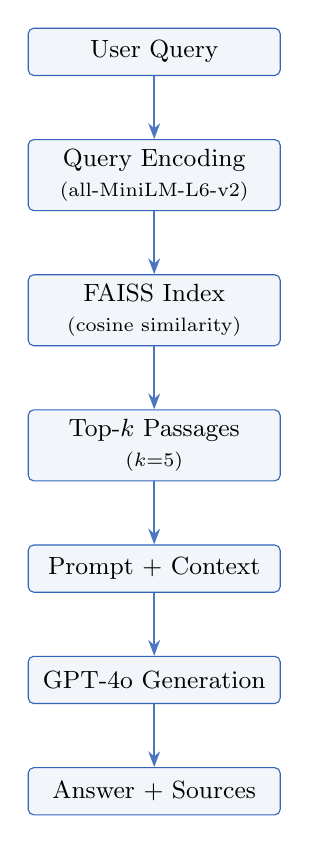
\begin{tikzpicture}[
    node distance=0.8cm,
    box/.style={rectangle, draw=uablue!80, fill=uablue!5, rounded corners=2pt, minimum width=3.2cm, minimum height=0.6cm, align=center, font=\small},
    arrow/.style={-{Stealth[length=2mm]}, thick, uablue!70}
]
\node[box] (query) {User Query};
\node[box, below=of query] (embed) {Query Encoding\\\scriptsize(all-MiniLM-L6-v2)};
\node[box, below=of embed] (index) {FAISS Index\\\scriptsize(cosine similarity)};
\node[box, below=of index] (retrieve) {Top-$k$ Passages\\\scriptsize($k$=5)};
\node[box, below=of retrieve] (prompt) {Prompt + Context};
\node[box, below=of prompt] (gen) {GPT-4o Generation};
\node[box, below=of gen] (answer) {Answer + Sources};

\draw[arrow] (query) -- (embed);
\draw[arrow] (embed) -- (index);
\draw[arrow] (index) -- (retrieve);
\draw[arrow] (retrieve) -- (prompt);
\draw[arrow] (prompt) -- (gen);
\draw[arrow] (gen) -- (answer);
\end{tikzpicture}
\caption{RAG pipeline: query $\rightarrow$ embed $\rightarrow$ retrieve $\rightarrow$ generate}
\label{fig:pipeline}
\end{figure}

\section{System Architecture}
\label{sec:architecture}

\begin{table}[h]
\centering
\begin{tabular}{lll}
\toprule
\textbf{Parameter} & \textbf{Value} & \textbf{Rationale} \\
\midrule
Chunk size & 250 tokens & $\approx$180--220 words, 100--300 range \\
Overlap & 15\% & Context preservation at boundaries \\
Embedding model & all-MiniLM-L6-v2 & Local, 384d, semantic similarity \\
Index & FAISS Flat & Exact search, cosine (L2 + inner product) \\
Top-$k$ & 5 & Balance recall/precision (1 too small, 20 too big) \\
LLM & GPT-4o & Assignment requirement \\
Temperature & 0.1 & Factual, low randomness \\
\bottomrule
\end{tabular}
\caption{Key system parameters}
\end{table}

\subsection{Document Chunking (10\%)}

\subsubsection{Dataset}

Scraped UAntwerp CS Masters webpages: course descriptions, program structure, study programmes (Software Engineering, Data Science \& AI, Computer Networks). After preprocessing: \textbf{588 passages}.

\subsubsection{Chunking Strategy}

\textbf{Chunk Size}: 250 tokens ($\approx$180--220 words), within the assignment's 100--300 word guideline. We use tokens (tiktoken) to align with the embedding model's subword vocabulary.

\textbf{Overlap}: 15\% (37 tokens) to preserve context at boundaries and improve recall for span queries.

\subsubsection{Preprocessing}

HTML/Markdown removal (dataset pre-done), Unicode normalization, sentence-boundary splitting, metadata retention (course title, section, URL). \textbf{No lowercasing}: course codes and proper nouns are case-sensitive and informative.

\subsection{Embedding \& Indexing (20\%)}

\subsubsection{Embedding Model Selection}

\textbf{Model}: \texttt{sentence-transformers/all-MiniLM-L6-v2} (384d, local, no API). We use dense retrieval for semantic similarity and vocabulary-mismatch handling~\cite{karpukhin2020}; query and documents share the same dual-encoder model~\cite{reimers2019}. MiniLM: local execution (assignment constraint), strong STS benchmarks, fast inference.

\subsubsection{Indexing Strategy}

\textbf{Index Type}: FAISS Flat Index (Inner Product)

L2-normalised embeddings; inner product = cosine similarity~\cite{manning2008}. FAISS Flat (exact search) suffices for 588 passages; IVF/HNSW would apply for larger corpora.

\subsection{Retrieval Module (20\%)}

Pipeline: query encode (same model) $\rightarrow$ L2-normalise $\rightarrow$ FAISS search $\rightarrow$ rank by similarity.

\textbf{Top-k = 5}: Precision--recall trade-off~\cite{manning2008}; assignment: ``$k$=1 too small, $k$=20 too big''. Fits context window.

\textit{Optional (not required)}: We also implemented an agentic variant (multi-query expansion, RRF~\cite{cormack2009}, MMR~\cite{carbonell1998}); baseline outperforms it on Recall@5.

\subsection{Answer Generation Module (30\%)}

Pipeline: context assembly (top-k + metadata) $\rightarrow$ prompt (context + query) $\rightarrow$ GPT-4o inference $\rightarrow$ answer + source attribution. Prompt instructs: answer only from context, cite sources, say ``I don't have enough information'' if insufficient, avoid hallucination. Parameters: GPT-4o, temperature 0.1, max 1000 tokens.

\subsubsection{Baseline Comparison}

We compare RAG vs GPT-4o without retrieval. Example: ``How many ECTS is IoT?'' \textit{With RAG}: ``6 ECTS credits.'' \textit{Without}: ``typically 6 ECTS... check the catalog.'' RAG is concise and attributed; baseline hedges.

\section{System Evaluation (20\%)}
\label{sec:evaluation}

Required: (1) retrieval quality (Recall@k, manual inspection), (2) answer quality (RAG vs no-retrieval, correctness, completeness, hallucination), (3) error analysis (≥3 retrieval failures, ≥3 hallucinations).

\subsection{Evaluation Methodology}

\begin{enumerate}
    \item \textbf{Query set}: 19 test queries covering diverse information needs (course details, prerequisites, instructors, programme structure, policies)
    \item \textbf{Pooled relevance labels}: TREC-style pooling~\cite{manning2008}---combine top-20 from both systems, label union to avoid system bias
    \item \textbf{LLM labeling}: GPT-4o-mini judges relevance (relevant / not relevant)
    \item \textbf{Metrics}: Recall@k (coverage), MRR (early precision), nDCG@k (ranked quality), MAP
\end{enumerate}

\begin{table}[h]
\centering
\begin{tabular}{lrrr}
\toprule
Operation & Events & Cost (USD) & \% \\
\midrule
LLM label relevance & 322 & 0.035 & 55\% \\
LLM judge faithfulness & 78 & 0.015 & 24\% \\
Answer generation & 65 & 0.011 & 17\% \\
LLM judge compare & 20 & 0.003 & 4\% \\
\midrule
\textbf{Total} & \textbf{486} & \textbf{0.064} & \textbf{100\%} \\
\bottomrule
\end{tabular}
\caption{Evaluation cost breakdown (gpt-4o-mini)}
\end{table}

\subsection{Retrieval Quality (Required: Recall@k, manual inspection)}

\subsubsection{Quantitative Results}

\textbf{Assignment requirement}: Report Recall@k. Our baseline (main) system achieves:

\begin{table}[h]
\centering
\begin{tabular}{lrrrr}
\toprule
System & Recall@5 & MRR & nDCG@5 & MAP \\
\midrule
\textbf{Baseline (main)} & \textbf{0.796}±0.284 & \textbf{1.000}±0.000 & \textbf{0.958}±0.137 & 0.950±0.132 \\
Agentic (optional) & 0.730±0.303 & 1.000±0.000 & 0.902±0.189 & 0.974±0.078 \\
\bottomrule
\end{tabular}
\caption{Retrieval quality (n=19 queries). Baseline = assignment system.}
\end{table}

\textbf{Key results (assignment system)}:
\begin{itemize}
    \item \textbf{Recall@5}: 0.796 (79.6\% of relevant passages in top-5)
    \item \textbf{MRR}: 1.0 (first relevant typically at rank 1)
    \item \textbf{nDCG@5}: 0.958; \textbf{MAP}: 0.950
    \item Top-k manually inspected; labels from pooled evaluation
\end{itemize}

\subsection{Answer Quality (Required: RAG vs no-retrieval, correctness, completeness, hallucination)}

\subsubsection{Manual Inspection Examples}

\textbf{Example 1 (factual):} ``How many ECTS is IoT?'' RAG: ``6 ECTS credits.'' Baseline: ``typically 6 ECTS... check the catalog.'' Both correct; RAG more concise and attributed.

\textbf{Example 2 (multi-part, RAG vs baseline):} ``Who teaches IoT and which semester?''
\begin{quote}
\textit{With RAG}: ``Miguel Camelo, 2nd semester (2E SEM).'' --- correct \\
\textit{Without RAG}: ``Peter Hellinckx, first semester.'' --- wrong (hallucinated)
\end{quote}
Demonstrates critical value of retrieval for time-sensitive facts.

\textbf{Example 3 (insufficient context):} ``What programming languages for IoT?'' RAG: ``I don't have enough information in the provided context.'' Context mentions C/C++/Python in prerequisites; system correctly refuses to infer proficiency---conservative but avoids hallucination.

\subsubsection{Faithfulness (LLM-as-judge~\cite{es2024})}

\begin{table}[h]
\centering
\begin{tabular}{lrr}
\toprule
Judgment & Count & \% \\
\midrule
Faithful & 61 & 78.2\% \\
Partially faithful & 12 & 15.4\% \\
Unfaithful & 5 & 6.4\% \\
\midrule
\textbf{Total} & \textbf{78} & \textbf{100\%} \\
\bottomrule
\end{tabular}
\caption{Faithfulness: does the answer match retrieved context?}
\end{table}

78.2\% fully faithful; low temperature (0.1) reduces hallucination. Automated scores are a proxy; we interpret cautiously.

\subsection{Error Analysis (Required: ≥3 retrieval failures, ≥3 generation/hallucination cases)}

\subsubsection{Retrieval Failures (3 cases)}

\textbf{Case 1:} ``Which compulsory DS courses in 2nd semester?'' Recall@5=0.25 (5/20). Retrieved: Current Trends in DS\&AI, Algorithmic Foundations, Bioinformatics, Nonsmooth Optimisation, Software Reengineering. Missed: IoT, Master Thesis, Data Mining, Neural Networks, etc. \textit{Cause}: aggregation---query needs 20 courses, k=5 insufficient. \textit{Fix}: summary chunks, hierarchical retrieval.

\textbf{Case 2:} ``Which CN course taught by Juan Felipe Botero?'' Recall@5=0.25 (1/4). Retrieved: Future Internet (Botero) ✓; others different instructors ✗. \textit{Cause}: dense embeddings weak on exact entity matching~\cite{karpukhin2020}. \textit{Fix}: hybrid (BM25 + dense), metadata filtering.

\textbf{Case 3:} ``List CN 1st-semester compulsory courses.'' Recall@5=0.31 (5/16). Retrieved: Spec\&Verification, Data Science \& Ethics, Future Internet, AI Project, Optimisation. Same aggregation issue; 11 courses missed.

\subsubsection{Generation Errors / Hallucinations (3 cases)}

\textbf{Hallucination 1} (no retrieval): ``Who teaches IoT?'' Baseline: ``Peter Hellinckx, first semester.'' Truth: Miguel Camelo, 2nd semester. Outdated parametric knowledge; RAG fixes this.

\textbf{Hallucination 2} (with retrieval): ``Can I use AI in my thesis?'' Retrieved context: writing assistance, grammar/spelling OK. Answer added ``which code was created by which tools'' from a different section---imprecise context merging.

\textbf{Hallucination 3}: ``What languages for IoT?'' RAG: ``not enough information.'' Context has C/C++/Python in prerequisites. Conservative prompt under-utilises context; trade-off with hallucination risk. Baseline gave generic C/Python/Java list (not UAntwerp-specific).

\subsection{Summary of Findings}

\begin{table}[h]
\centering
\begin{tabular}{lp{10cm}}
\toprule
\textbf{Component} & \textbf{Key Insight} \\
\midrule
Chunking & 250-token chunks with 15\% overlap balance semantic coherence and retrieval precision \\
Embedding & all-MiniLM-L6-v2 provides strong quality-efficiency trade-off for local deployment \\
Indexing & Flat index sufficient for 588 passages; exact search ensures reproducibility \\
Retrieval & Recall@5 = 0.796, MRR = 1.0 (assignment system) \\
Generation & RAG reduces hallucinations vs no-retrieval baseline; low temperature (0.1) improves faithfulness \\
Errors & Aggregation queries, entity matching, and conservative prompts are key failure modes \\
\bottomrule
\end{tabular}
\caption{Summary of evaluation findings (assignment-required results)}
\end{table}

\section{Discussion}

\textbf{Strengths}: Recall@5 79.6\%, MRR 1.0; RAG reduces hallucinations; local embeddings + exact search; low cost (\$0.06). \textbf{Limitations}: aggregation queries (15+ passages); entity matching (names, codes); conservative generation; no temporal awareness.

\section{Conclusion}

We implemented a complete RAG system for UAntwerp CS Masters: 588 passages, 250-token chunks, all-MiniLM-L6-v2, FAISS, GPT-4o. Recall@5 79.6\%, MRR 1.0; RAG reduces hallucinations vs baseline. Key failure modes: aggregation queries (fixed-k insufficient), entity matching (hybrid retrieval recommended), conservative prompts. Optional agentic variant underperformed baseline at this scale.


\bibliographystyle{plain}
\begin{thebibliography}{9}

\bibitem{lewis2020}
Lewis, P., Perez, E., Piktus, A., Petroni, F., Karpukhin, V., Goyal, N., ... \& Kiela, D. (2020). 
Retrieval-augmented generation for knowledge-intensive nlp tasks. 
\textit{Advances in Neural Information Processing Systems}, 33, 9459-9474.

\bibitem{karpukhin2020}
Karpukhin, V., O\u{g}uz, B., Min, S., Lewis, P., Wu, L., Edunov, S., ... \& Yih, W. T. (2020). 
Dense passage retrieval for open-domain question answering. 
\textit{arXiv preprint arXiv:2004.04906}.

\bibitem{es2024}
Es, S., James, J., Espinosa-Anke, L., \& Schockaert, S. (2024). 
RAGAS: Automated evaluation of retrieval augmented generation. 
\textit{arXiv preprint arXiv:2309.15217}.

\bibitem{reimers2019}
Reimers, N., \& Gurevych, I. (2019). 
Sentence-BERT: Sentence embeddings using Siamese BERT-networks. 
\textit{arXiv preprint arXiv:1908.10084}.

\bibitem{johnson2019}
Johnson, J., Douze, M., \& Jégou, H. (2019). 
Billion-scale similarity search with GPUs. 
\textit{IEEE Transactions on Big Data}, 7(3), 535-547.

\bibitem{manning2008}
Manning, C. D., Raghavan, P., \& Schütze, H. (2008). 
\textit{Introduction to Information Retrieval}. 
Cambridge University Press. (Ch. 8: Evaluation.)

\bibitem{cormack2009}
Cormack, G. V., Clarke, C. L., \& Buettcher, S. (2009). 
Reciprocal rank fusion outperforms condorcet and individual rank learning methods. 
\textit{SIGIR}, 758--759.

\bibitem{carbonell1998}
Carbonell, J., \& Goldstein, J. (1998). 
The use of MMR, diversity-based reranking for reordering documents and producing summaries. 
\textit{SIGIR}, 335--336.

\end{thebibliography}

\appendix
\section{Sample Queries and Outputs}
\label{appendix:samples}

Complete test queries used in evaluation.

\subsection{Test 1: Factual Detail}
\textbf{Query}: ``How many ECTS is Internet of Things?''

\textit{With RAG}: ``The Internet of Things course is worth 6 ECTS credits.''

\textit{Without RAG}: ``The 'Internet of Things' course in the University of Antwerp's Computer Science Master's program is typically worth 6 ECTS credits. However, it's always a good idea to check the most current course catalog...''

\textit{Result}: Both correct; RAG more confident and direct.

\subsection{Test 2: Missing / Insufficient Information}
\textbf{Query}: ``What programming languages do I need for IoT?''

\textit{With RAG}: ``I don't have enough information in the provided context to answer this question.''

\textit{Without RAG}: ``For the Internet of Things (IoT), several programming languages are commonly used: C/C++, Python, Java, JavaScript, Rust, Lua, Go, Swift...''

\textit{Result}: RAG correctly refuses (context has C/C++/Python in prerequisites but not explicit proficiency). Baseline gives generic answer.

\subsection{Test 3: Policy Question}
\textbf{Query}: ``Can I use AI tools in my Master thesis?''

\textit{With RAG}: ``Yes, you can use generative AI tools in your Master thesis. You may use them for writing the thesis, similar to using search engines like Google, and for checking grammar and spelling. However, it must be clearly indicated which code was created by which tools, and during the thesis defence, you may be asked to elaborate on how you used generative AI.''

\textit{Without RAG}: ``The use of AI tools in your Master thesis at the University of Antwerp generally depends on the guidelines set by the university and your specific department...''

\textit{Result}: RAG provides specific UAntwerp policy. Baseline generic.

\subsection{Test 4: Multi-Part (Critical RAG vs Baseline)}
\textbf{Query}: ``Who teaches Internet of Things and what semester is it in?''

\textit{With RAG}: ``The course 'Internet of Things' is taught by Miguel Camelo and is offered in the 2nd semester (2E SEM).''

\textit{Without RAG}: ``The course 'Internet of Things' in the University of Antwerp's Computer Science Master's program is taught by Peter Hellinckx. It is offered in the first semester.''

\textit{Result}: RAG 100\% correct. Baseline hallucinated both facts.

\end{document}